\documentclass[runningheads]{llncs}
\usepackage{graphicx}
\usepackage{booktabs}
\usepackage{amsmath,amssymb}
\usepackage{microtype}
\usepackage{url}
\usepackage{enumitem}
\usepackage{cite}
\newcommand{\ClinicalDeltaLow}{-0.002}
\newcommand{\ClinicalDeltaHigh}{0.102}
\newcommand{\CarfAuc}{0.849}
\newcommand{\AnchorAuc}{0.802}
\newcommand{\NoRobustAuc}{0.871}
\newcommand{\StackAuc}{0.851}
\newcommand{\CarfInternal}{0.731}
\newcommand{\StackInternal}{0.747}
\newcommand{\RnaBudget}{0.732}
\newcommand{\MriBudget}{0.268}
\newcommand{\TotalBudget}{1.000}
\newcommand{\RnaPermCarf}{0.785}
\newcommand{\RnaPermNoRobust}{0.753}
\newcommand{\MriPermCarf}{0.838}
\newcommand{\MriPermNoRobust}{0.860}
\newcommand{\CertifiedPairs}{14.270}
\newcommand{\RppaThreeAuc}{0.761}
\newcommand{\RppaFourAuc}{0.733}
\newcommand{\CommonGenes}{16,637}

\titlerunning{Clinical-Anchored Residual Fusion}
\title{Bounded Clinical-Anchored Residual Fusion for Multimodal Prediction under Modality Failure}
\author{Anonymous Author(s)}
\institute{Institution withheld for double-blind review}
\begin{document}
\maketitle
\begin{abstract}
Optional modalities can improve prediction but also introduce acquisition-specific failure. We propose clinical-anchored residual fusion (CARF), which lets transcriptomic and MRI experts correct a clinical predictor within a learned log-odds budget. Six nonnegative coefficients combine clipped residuals with bounded agreement/confidence features. A convex objective trains on out-of-fold predictions across availability and corruption environments. The architecture guarantees exact clinical fallback when optional inputs are absent and bounds each modality's influence, without guaranteeing accuracy. We evaluate 976 I-SPY2 and 112 I-SPY1 participants using 25 internal folds, matched ablations, and repeated stress tests. External AUROC is \CarfAuc{} versus \AnchorAuc{} for clinical-only and \StackAuc{} for stacking. The paired gain over clinical-only has 95\% interval $[\ClinicalDeltaLow,\ClinicalDeltaHigh]$. Removing robust loss gives higher clean AUROC (\NoRobustAuc{}) but poorer RNA-permutation robustness. The contribution is a constrained formulation with verifiable stability properties and a reproducible evaluation. Earlier external findings informed development; independent confirmation remains necessary.
\keywords{Multimodal learning \and Missing modalities \and Robust fusion \and Convex optimization}
\end{abstract}

\section{Introduction}
Pretreatment prediction of pathological complete response (pCR) tests multimodal learning under acquisition and cohort shift. MRI measures contrast enhancement and morphology, microarrays measure expression, and clinical records capture age and receptor status. An expert useful in one cohort may fail in another. Unconstrained stacking can amplify that failure, while confidence features alone provide no influence guarantee: an incorrect expert can be highly confident.

We ask whether optional acquisitions can contribute useful corrections while their maximum influence remains explicit. CARF retains the clinical logit as an offset and learns bounded molecular/MRI residuals. Clinical availability is an operational assumption, and anchor selection was informed by the project's earlier external findings.

Our contributions are (1) an explicit correction budget with fallback, perturbation bounds, and ranking certificates; (2) a convex objective over missingness and corruption environments; and (3) a matched evaluation with corrected fold-contained preprocessing, architectural ablations, uncertainty, and stress tests. We do not claim state-of-the-art performance or priority for the general idea of anchored fusion.

\section{Related Work and Scope}
Multimodal learning combines heterogeneous signals \cite{baltrusaitis2019}; biomedical settings add acquisition variability and incomplete measurements \cite{acosta2022}. ModDrop trains with dropped channels \cite{neverova2015}. CARF enumerates the four optional-modality masks while retaining a mandatory anchor.

QA-MoE separates quality estimation from expert routing for noisy and missing clinical inputs \cite{sun2026}. UCMR-Net uses a text anchor with adaptive nonverbal residuals \cite{tang2026}. CARF's proposed distinction is the constrained logit correction, separable bounded context basis, and convex cross-fitted objective, not generic reliability weighting or an anchor plus residuals. Recent diagnostics question whether reliability scores influence decisions usefully \cite{moon2026}; our constant-basis ablation tests their incremental value. We do not claim to reproduce these neural architectures experimentally.

Worst-group optimization emphasizes poorly performing environments \cite{sagawa2020}. Our environments instead perturb optional-expert probabilities, not demographic groups or observed deployment sites. The smooth worst-environment objective addresses this specified family. The influence bound is architectural and applies to arbitrary optional values; neither statement guarantees generalization under arbitrary clinical shift.

\section{Data and Fold-Contained Preprocessing}
\subsection{Patient-linked acquisitions}
We use I-SPY2 for development and I-SPY1 for exploratory cross-cohort evaluation. TCIA provides the I-SPY imaging collections \cite{tciaispy1,tciaispy2}; the acquired BreastDCEDL archives contain pretreatment cropped contrast phases and supplied tumour masks \cite{fridman2026}. Expression comes from GEO GSE194040 for I-SPY2 and GSE22226 for I-SPY1. These are microarrays, not RNA sequencing. The I-SPY2 molecular resource also provides RPPA through GSE196093 \cite{wolf2022ispy}.

Identifiers are matched explicitly across acquisitions. Technical expression replicates are averaged after response agreement checks. Source outcome conflicts, unmatched identifiers, and image quality failures are recorded in the linkage and image audits. The complete-case analysis contains 976 I-SPY2 participants (315 pCR) and 112 I-SPY1 participants (31 pCR). Only pretreatment features enter models. Treatment follow-up, response variables, survival endpoints, treatment arm, and publisher train/test indicators are excluded from predictors. This pooled prediction task does not estimate treatment-specific causal effects.

\subsection{Molecular and clinical transformations}
We intersect annotated gene symbols across assay platforms, retaining \CommonGenes{} common genes before learned selection. For each patient separately, expression is transformed to average ranks among observed finite genes divided by their patient-specific observed count; missing entries remain missing until training-fitted imputation. This transformation does not estimate external cohort moments or use outcome labels. It does use knowledge of external assay availability, and public assay preprocessing remains outside the scope of this reanalysis.

Every transcriptomic expert fit independently median-imputes its training inputs, selects the 3,000 highest-variance genes, selects up to 250 genes by training-label ANOVA, standardizes, and fits regularized logistic regression. The variance filter is fitted again inside every inner and outer training partition; held-out patient values do not determine it. The clinical expert uses age, hormone-receptor status, and HER2 with training-fitted median imputation and standardization. Numeric receptor indicators need no learned categorical vocabulary.

\subsection{Image features}
The MRI expert uses 66 fixed features extracted from precontrast, early postcontrast, and late postcontrast volumes. These phases are within a pretreatment examination, not longitudinal treatment response scans. Input checks cover image/mask shape agreement, finite tumour signal, sufficient mask size, physical spacing, and source-mask validity. Signal normalization uses the patient's positive precontrast median. Relative enhancement and late change divide by a stabilized absolute precontrast signal.

Features comprise 54 signal summaries, six geometric descriptors, two kinetic fractions, and four fixed-bin texture descriptors. The geometric descriptors are log volume, log surface area, bounding-box extent, sphericity, axis ratio, and log maximum extent. Texture uses symmetric masked nearest-neighbour enhancement co-occurrences. These are custom, outcome-independent features, not a claim of IBSI compliance. Supplied masks are annotations; automatic segmentation performance is not evaluated.

\section{Clinical-Anchored Residual Fusion}
\subsection{Experts and explicit missingness}
Let $p_C$ be the mandatory clinical probability, and $p_R,p_M$ optional transcriptomic and MRI probabilities. Experts use class-balanced logistic regression with $C=0.1$ for transcriptomics and $C=1$ for clinical/MRI. All choices are fixed for this revision. Probabilities are clipped to $[10^{-7},1-10^{-7}]$ before taking logits. Define the anchor $a=\operatorname{logit}(p_C)$, availability $m_j\in\{0,1\}$, and residual
\begin{equation}
 d_j=\operatorname{logit}(p_j)-a,\qquad
 r_j=\operatorname{clip}(d_j,-B,B),\qquad j\in\{R,M\}.
\end{equation}
Missing optional inputs are represented by explicit masks (NaN in the interface). A probability of $0.5$ means an observed neutral expert and is not interpreted as absence. Missing clinical predictions are rejected rather than silently imputed by the fusion layer.

\begin{figure}[t]
\centering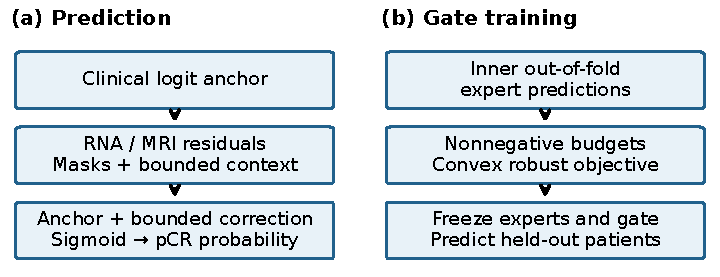
\includegraphics[width=\linewidth]{figures/carf_architecture.pdf}
\caption{(a) CARF prediction: the clinical logit is the anchor; optional experts contribute masked, bounded residual corrections. (b) Gate training uses inner out-of-fold predictions; frozen experts and gate predict outer or external patients.}
\label{fig:architecture}
\end{figure}

\subsection{Contextual correction budget}
Each optional expert has three bounded basis functions:
\begin{equation}
 h_{j0}=1,\qquad h_{j1}=e^{-|d_j|},\qquad
 h_{j2}=1-H(p_j)/\log 2,
\end{equation}
where $H(p)=-p\log p-(1-p)\log(1-p)$. All $h_{jk}$ lie in $[0,1]$. Agreement attenuates large logit differences, while confidence allows a different correction profile for decisive experts. Neither asserts that agreement or confidence implies correctness.
The fused predictor is
\begin{equation}
 z_\theta=a+\sum_{j\in\{R,M\}}\sum_{k=0}^{2}
 \theta_{jk}m_jh_{jk}r_j,\qquad
 \hat p=\sigma(z_\theta),\quad
 \theta_{jk}\geq0,\quad\sum_{j,k}\theta_{jk}\leq1.
 \label{eq:carf}
\end{equation}
There are six learned gate coefficients. Unused coefficient mass leaves more of the decision with the anchor. The architecture can suppress an optional expert but cannot reverse the sign of its residual correction. This restriction trades flexibility for interpretability and a uniform influence limit.

\subsection{Properties and limitations of the guarantee}
Write $b_j=B\sum_k\theta_{jk}$ and $b=\sum_j b_j\leq B$.
\textbf{Proposition 1 (fallback and bounded displacement).} If both optional experts are absent, $z_\theta=a$. For any optional probabilities and masks, $|z_\theta-a|\leq b$. Thus $|\hat p-p_C|\leq b/4$ relative to the clipped clinical probability.
\emph{Proof.} Missing inputs zero their summands. Otherwise $|m_jh_{jk}r_j|\leq B$, and the triangle inequality gives the logit bound. The sigmoid derivative is at most $1/4$.\hfill$\square$

\textbf{Proposition 2 (single-modality replacement).} Holding the anchor and other inputs fixed, arbitrary replacement or removal of modality $j$ changes the fused logit by at most $2b_j$ and probability by at most $b_j/2$.
\emph{Proof.} Only the $j$-indexed features change, because each context basis depends on its own expert and the anchor. Each old/new modality contribution belongs to $[-b_j,b_j]$.\hfill$\square$

A useful corollary is a label-free ranking certificate: two patients whose clinical logits differ by more than $2b$ retain that clinical ordering for any optional inputs. This certifies stability of an ordering, not its correctness. Bounds do not prevent a bad clinical anchor, do not guarantee improved AUROC, and do not cover corruption of the mandatory clinical modality. Exact fallback applies to the existing full model with absent inputs; removing a modality and retraining the remaining gate is a different ablation.

\subsection{Convex robust gate fitting}
Expert probabilities for gate fitting are generated by five-fold cross-fitting within the current training partition. Let $L_e(\theta)$ denote mean binary log loss in environment $e$. The four mask environments $\mathcal M$ contain all combinations of optional availability. Four corruption environments $\mathcal C$ replace one optional expert at a time by $0.01$ or $0.99$, leaving the clinical anchor and other expert unchanged. The objective is
\begin{equation}
 \min_{\theta\geq0,\,\mathbf1^\top\theta\leq1}
 \frac1{4}\sum_{e\in\mathcal M}L_e(\theta)
 +\gamma\tau\log\left(\frac1{4}\sum_{e\in\mathcal C}e^{L_e(\theta)/\tau}\right)
 +\frac\lambda2\|\theta\|_2^2.
 \label{eq:objective}
\end{equation}
Gate loss is unweighted even though experts use class balancing. We fix $B=1$, $\gamma=0.25$, $\tau=0.05$, and $\lambda=0.01$. There is no external hyperparameter search. The normalized smooth maximum lies between the worst environment loss minus $\tau\log4$ and that worst loss. Features and anchor logits are fixed during gate optimization; logistic loss is convex in $\theta$, as are the smooth maximum and regularizer. The feasible set is convex and compact; positive $\lambda$ makes the objective strictly convex. SLSQP solves the six-variable program with analytic gradients, and unsuccessful convergence aborts evaluation. This is a convex gate, not a claim of joint convexity across trainable experts.

\section{Evaluation Protocol}
\subsection{Matched comparisons and ablations}
The primary comparison shares the same expert predictions across all gates. Baselines are each expert alone, available-expert averaging, class-balanced probability stacking, and no-MRI stacking. We also fit mask-augmented logistic stacking on all four masks, with missing probabilities replaced by $0.5$ and three availability indicators. Each augmented row receives weight $1/4$, preserving the total training weight.

CARF ablations remove the robust loss ($\gamma=0$), remove patient context (constant basis only), remove both residual clipping and the coefficient-sum bound, or remove MRI before refitting. Other settings remain fixed. The unbounded variant retains nonnegative coefficients and regularization; it tests the combined influence constraint rather than isolating its two components. Missing-modality stress uses the trained full model, whereas the no-MRI ablation is trained without MRI. These are intentionally separate estimands.

\subsection{Cross-validation, uncertainty, and stress}
Internal evaluation uses five repeats of stratified five-fold cross-validation. In each outer training set, inner cross-fitting produces gate-training probabilities. Experts are then refitted on the outer training patients and predict the held-out fold. No held-out labels enter preprocessing, experts, or gates. We report mean fold AUROC descriptively; overlapping folds are not independent observations for a significance test. External fitting uses all I-SPY2 patients with the same inner protocol.

All models are assessed on the same I-SPY1 patients with AUROC, average precision (AP), Brier score, and log loss. Paired percentile bootstrap intervals use 2,000 patient resamples for the CARF-minus-comparator AUROC difference. They describe uncertainty conditional on fitted models, not uncertainty in model selection or training. Multiple exploratory comparisons are not treated as confirmatory tests.

Stress tests freeze every fitted model and modify optional-expert outputs only. Conditions include explicit absence, neutralization at $0.5$, extreme replacement, patient permutation, and clipped Gaussian noise with standard deviation $0.25$. Noise and permutation are repeated with 30 fixed seeds per optional modality. These interventions isolate fusion behavior; they do not simulate raw-image scanner physics, segmentation errors, or the prevalence of clinical failures. Mean stress AUROC and prediction displacement are reported separately.

\subsection{Corrections and exploratory status}
This revision corrects three earlier defects: gene variance filtering before internal splitting, expert fitting within RPPA test partitions, and rank normalization that erased an entire expression row when one gene was missing. The latter caused constant external RNA predictions. All comparisons are rerun with observed-gene ranks, training-fitted imputation, and strictly separated fit/predict partitions. Earlier gate-only label permutations retained outcome-trained experts and are excluded as invalid whole-pipeline null tests.

Earlier I-SPY1 findings were visible during CARF design. Although external labels enter neither fitting nor numerical hyperparameter selection, the analysis is exploratory rather than an untouched-test evaluation. Historical artifacts remain separate for traceability.

\section{Results}
\subsection{Discrimination and matched ablations}
\begin{table}[t]
\centering\caption{Matched comparisons. Internal AUC is the mean over 25 outer folds; external metrics use 112 I-SPY1 participants. AP denotes average precision.}
\small\setlength{\tabcolsep}{4pt}\begin{tabular}{lrrrr}
\toprule
Model & CV AUC & Ext. AUC & Ext. AP & Brier\\
\midrule
Transcriptomic & 0.723 & 0.809 & 0.659 & 0.178\\
Clinical anchor & 0.662 & 0.802 & 0.617 & 0.205\\
MRI & 0.629 & 0.607 & 0.360 & 0.314\\
Available-expert mean & 0.751 & 0.837 & 0.649 & 0.167\\
Probability stacking & 0.747 & 0.851 & 0.667 & 0.151\\
No-MRI stacking & 0.733 & 0.853 & 0.694 & 0.148\\
Mask-augmented stacking & 0.746 & 0.859 & 0.672 & 0.148\\
CARF (proposed) & 0.731 & 0.849 & 0.699 & 0.173\\
CARF: no robust loss & 0.743 & 0.871 & 0.713 & 0.146\\
CARF: constant basis & 0.733 & 0.850 & 0.692 & 0.172\\
CARF: unbounded residual & 0.725 & 0.851 & 0.691 & 0.174\\
CARF: no MRI & 0.718 & 0.842 & 0.668 & 0.171\\
\bottomrule
\end{tabular}

\label{tab:performance}
\end{table}
Table~\ref{tab:performance} retains every planned comparison, including ablations. CARF achieves external AUROC \CarfAuc{}, compared with \AnchorAuc{} for the clinical anchor, and \StackAuc{} for ordinary probability stacking. Its mean internal AUROC is \CarfInternal{}, compared with \StackInternal{} for stacking. A point-estimate difference is not sufficient evidence of superiority; the paired intervals in Table~\ref{tab:paired} determine the precision available from this external sample.

\begin{table}[t]
\centering\caption{Paired external AUROC differences, CARF minus comparator. Percentile intervals use 2,000 patient bootstrap resamples and are conditional on the fitted predictors.}
\begin{tabular}{lrr}
\toprule
Comparator & $\Delta$AUROC & 95\% interval\\
\midrule
Clinical anchor & +0.047 & [-0.002, +0.102]\\
Probability stacking & -0.001 & [-0.060, +0.058]\\
Mask-augmented stacking & -0.010 & [-0.059, +0.037]\\
CARF: no MRI & +0.007 & [-0.031, +0.044]\\
\bottomrule
\end{tabular}

\label{tab:paired}
\end{table}
The no-robust-loss ablation reaches external AUROC \NoRobustAuc{}, the largest clean point estimate among the predefined models. It is retained as an ablation rather than promoted after external inspection. The constant-basis ablation is also competitive with full CARF; these results do not establish that the context channels improve discrimination. Thus the mathematical influence guarantee is better supported than a claim that every component improves clean accuracy.

Class-balanced experts may be miscalibrated to cohort prevalence. Brier scores therefore complement ranking metrics; log losses are retained in the result files. CARF inherits the clinical offset and supplies no separate calibration guarantee.

\subsection{Modality failure and learned influence}
\begin{table}[t]
\centering\caption{External AUROC under frozen-model stress. Random noise and permutation entries average 30 realizations. For ordinary stacking, absent inputs are replaced by 0.5; mask stacking and CARF receive explicit availability.}
\small\setlength{\tabcolsep}{3pt}\begin{tabular}{lrrrrr}
\toprule
Condition & Clinical & Stack & Mask & CARF & No robust\\
\midrule
intact & 0.802 & 0.851 & 0.859 & 0.849 & 0.871\\
rna missing & 0.802 & 0.750 & 0.781 & 0.795 & 0.796\\
mri missing & 0.802 & 0.854 & 0.857 & 0.840 & 0.863\\
both missing & 0.802 & 0.802 & 0.802 & 0.802 & 0.802\\
rna permuted & 0.802 & 0.689 & 0.728 & 0.785 & 0.753\\
mri permuted & 0.802 & 0.804 & 0.832 & 0.838 & 0.860\\
rna noisy & 0.802 & 0.806 & 0.828 & 0.831 & 0.841\\
mri noisy & 0.802 & 0.830 & 0.846 & 0.847 & 0.866\\
\bottomrule
\end{tabular}

\label{tab:stress}
\end{table}
The fitted CARF logit budgets are \RnaBudget{} for transcriptomics and \MriBudget{} for MRI, with total \TotalBudget{}. Across the external patients, \CertifiedPairs{}\% of all unordered clinical-score pairs have anchor separation greater than twice the learned total budget. Their clinical ordering is invariant to optional-input replacement under this fitted model. This certificate does not use outcome labels and does not certify correct classification.

The robust objective exposes a modality-dependent tradeoff. Under RNA permutation, CARF averages AUROC \RnaPermCarf{} versus \RnaPermNoRobust{} without the robust loss. Under MRI permutation, the corresponding values are \MriPermCarf{} and \MriPermNoRobust{}. The robust loss therefore does not dominate its ablation across failures: it sacrifices clean discrimination and improves resistance to corrupted molecular ordering, while the simpler bounded variant remains stronger under MRI permutation. These are descriptive averages over perturbations, not statistical tests over new patients.

When both optional inputs are absent, CARF returns the clipped clinical probability. Table~\ref{tab:stress} separates empirical discrimination from the structural displacement guarantee.

\begin{figure}[t]
\centering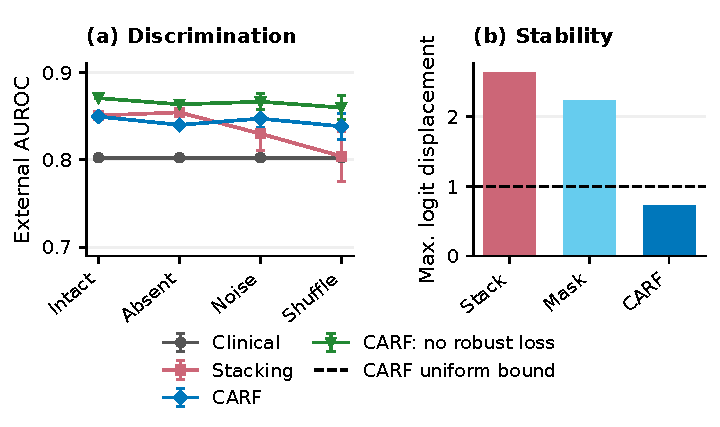
\includegraphics[width=\linewidth]{figures/carf_stress.pdf}
\caption{(a) External MRI stress, with standard deviations across random corruption realizations (not patient-sampling confidence intervals). (b) Largest observed anchor displacement across intact, noisy-MRI, and permuted-MRI evaluations, compared with CARF's learned uniform bound.}
\label{fig:stress}
\end{figure}

\subsection{Secondary protein extension}
The patient-linked RPPA subset contains 728 I-SPY2 participants and 139 protein features. In five matched stratified folds, a conventional three-expert stack has mean AUROC \RppaThreeAuc{}, while adding imputed, standardized RPPA features to its gate yields \RppaFourAuc{}. Held-out probabilities now come exclusively from experts fitted on the corresponding training partition. This is a secondary feature-level extension, not a fourth CARF expert and not external protein validation. Its subset, architecture, and evaluation differ from the primary experiment, so its performance is not directly comparable to the full-cohort table.

\section{Discussion and Limitations}
CARF bounds optional inputs while allowing corrections that vary across patients and convex gate fitting. Its guarantees concern stability, not accuracy. A useful but discordant expert may be underweighted, negative residual weights are forbidden, and no guarantee covers clinical-anchor failure. Context and robust-loss ablations do not uniformly improve discrimination. Tuned nonlinear and neural baselines remain necessary before claiming competitive superiority.

Only 112 external participants and 31 positive outcomes are available. Platforms, treatments, case mix, and imaging provenance differ. Complete-case selection can bias evaluation, and synthetic missingness does not establish performance on naturally absent acquisitions. Public assay preprocessing and supplied masks limit deployment claims. Repeated folds are dependent, and bootstrap intervals omit fitting uncertainty. Since earlier I-SPY1 outcomes informed development, the next decisive test is a frozen evaluation on an independent cohort.

\section{Reproducibility and Conclusion}
The repository provides source/input hashes, optimizer diagnostics, all fold predictions, stress realizations, bootstrap samples, tests, and generated tables. The Makefile provides analysis, validation, asset-generation, and paper targets; exact commands are in the README. Source MRI manifests and patient-linkage audits document the processed inputs.

CARF offers bounded, mask-aware correction with convex training and provable fallback and influence properties. The matched experiments identify both useful behavior and accuracy--robustness tradeoffs. They support an exploratory methodological contribution, not established clinical utility or universal superiority.

\bibliographystyle{splncs04}
\bibliography{references}
\end{document}
